\documentclass[a0,portrait]{a0poster}

\usepackage{multicol}
\columnsep=100pt
\columnseprule=3pt

\usepackage{times}
\usepackage{graphicx}
\graphicspath{{../}}
\usepackage{booktabs}
\usepackage[font=small,labelfont=bf]{caption}
\usepackage{amsfonts, amsmath, amsthm, amssymb, marvosym}
\usepackage{wrapfig}
\usepackage{enumitem}
\usepackage{fancyvrb}
\usepackage{xspace}
\usepackage[svgnames,usenames,dvipsnames]{xcolor}
\usepackage{algorithm}
\usepackage[noend]{algorithmic}

\renewcommand{\algorithmicrequire}{\textbf{Input:}}
\renewcommand{\algorithmicensure}{\textbf{Output:}}
\newcommand{\cetable}{CE~}

\newcommand{\as}{AgentSpeak\xspace}
\newcommand{\Jason}{\emph{Jason}\xspace}
\newcommand{\pa}{planner agent\xspace}
\newcommand{\ia}{interface agent\xspace}
\newcommand{\pas}{planner agents\xspace}
\newcommand{\ias}{interface agents\xspace}
\newcommand{\PA}{Planner Agent\xspace}
\newcommand{\IA}{Interface Agent\xspace}
\newcommand{\Pa}{Planner agent\xspace}
\newcommand{\Ia}{Interface agent\xspace}
\newcommand{\Pas}{Planner agents\xspace}
\newcommand{\Ias}{Interface agents\xspace}

\def\texttts#1{\texttt{\large#1}}

\begin{document}

%---------------------------------------------------------------
%	POSTER HEADER 
%---------------------------------------------------------------
\begin{minipage}[b]{0.75\linewidth}
\veryHuge \color{NavyBlue} 
\textbf{TITULO} 
\color{Black}\\[2cm] % Subtitle
\huge \textbf{Matheus de Souza Redecker e Felipe Meneguzzi}\\
\Large Faculdade de Inform\'atica (FACIN) -- 
Pontif\'icia Universidade Cat\'olica do Rio Grande do Sul (PUCRS)\\ 
Porto Alegre -- RS -- Brasil\\ % University/organization
\Large \Letter ~ \texttt{matheus.redecker@acad.pucrs.br}\\
\Large \Letter ~ \texttt{felipe.meneguzzi@pucrs.br}\\
\\
% \Telefon ~ \large \texttt{+55\,(51)\,3353-8627}\\
\end{minipage}
\hspace*{-2cm}
\begin{minipage}[t]{0.25\linewidth}
\begin{center}
\vspace{-12cm}

\includegraphics[width=9cm]{logoPUCRS.pdf}%\\[-0.8cm]
\hspace*{1cm}
\end{center}
\end{minipage}

%---------------------------------------------------------------

\begin{multicols}{2} 
%---------------------------------------------------------------
%	ABSTRACT
%---------------------------------------------------------------
\color{NavyBlue}
\color{Black}
\raggedright
\Large

\newcommand\itemadjust{\itemsep.5em \parskip0pt \parsep0pt}
%---------------------------------------------------------------
%	INTRODUCTION
%---------------------------------------------------------------
\color{NavyBlue}
\section*{\huge Motiva\c{c}\~ao}
\color{Black}

%[leftmargin=2em]\itemadjust
\begin{itemize}
	\item Qual o problema?;
	\item Pq é interessante?; e
	\item O que tu te propoe a fazer?
\end{itemize}

%---------------------------------------------------------------
%   APPROACH
%---------------------------------------------------------------
\color{NavyBlue}
\section*{\huge Background}
\color{Black}

\textbf{AHTN(escrever o nome inteiro)}

\begin{itemize}
	\item dasid
	\item ehaushe
\end{itemize}

\vspace{10mm}
\textbf{MicroRTS com figuras}


\begin{itemize}
	\item O MicroRTS é um jogo de estrategia em tempo real(RTS);
	\item Ele é uma simplificação do jogo Starcraft, feito por Santiago Ontañón \cite{ontanon2013combinatorial};
	\item O MicroRTS foi desenvolvido para fins acadêmicos, com o intuito de aplicar e desenvolver técnicas de IA e para servir como prova de conceito para as técnicas criadas.
\end{itemize}

\begin{center}
	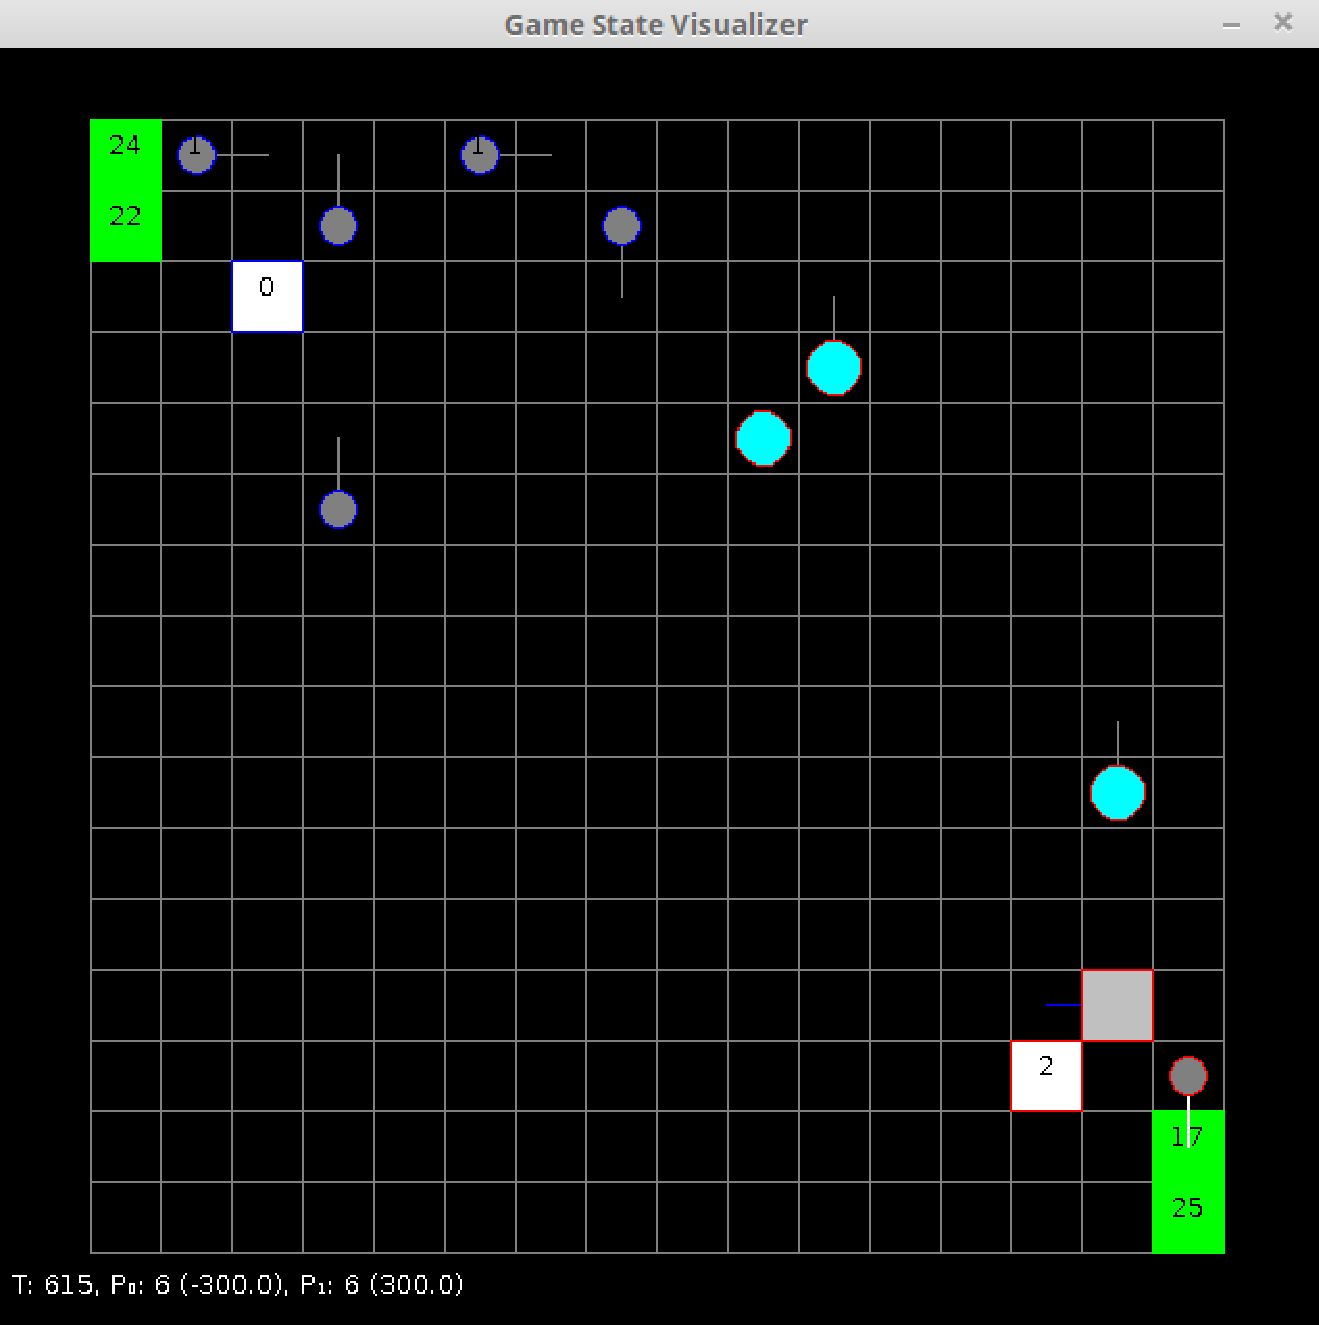
\includegraphics[width=0.6\linewidth]{microRts.pdf}
	\captionof{figure}{Exemplo de tela de um jogo do MicroRTS.}
\end{center}	


%---------------------------------------------------------------
%	Implementação
%---------------------------------------------------------------
\color{NavyBlue}
\section*{\huge Implementa\c{c}\~ao}
\color{Black}

Falar alguma coisa aqui

\vspace{10mm}

\begin{itemize}
	\item Conhecimento de dominio
\end{itemize}


%---------------------------------------------------------------
%	EXPERIMENTS AND RESULTS
%---------------------------------------------------------------
\color{NavyBlue}
\section*{\huge Experimentos e resultados}
\color{Black}

\begin{itemize}
	\item graficozinhos
\end{itemize}


\vspace{13mm}



%---------------------------------------------------------------
%	CONCLUSION
%---------------------------------------------------------------
\vspace{-12mm}
\color{NavyBlue}
\section*{\huge Conclus\~ao}
\color{Black}

We have shown empirically that our approach yields not only superior accuracy results but also substantially faster recognition times for all used domains in evaluating against Ram{\'{\i}}rez and Geffner's approach~\cite{RamirezG_IJCAI2009}.

%\begin{itemize}[leftmargin=2em]\itemadjust
%	\item This work addresses the gap in existing norm identification approaches, which assume that violations do not occur, or that when they occur a violation signal is always generated
%	\item We consider two types of evidence:
%	\begin{itemize}
%		%\item Behaviour that is not necessarily always compliant
%                \item Observed traces of other agents, assumed to be generated by plans
%		\item Violation signals, which may be emitted following norm violation
%	\end{itemize}
%	\item An agent using our approach generates norm-compliant behaviour at least $70\%$ in the presence of a large number of norms
%\end{itemize}

%---------------------------------------------------------------
%	REFERENCES
%---------------------------------------------------------------
\vspace{-9mm}
\large
\color{NavyBlue}
\color{Black}
\raggedright
\bibliographystyle{plain}
\bibliography{poster}

\end{multicols}
%---------------------------------------------------------------
%	ACKNOWLEDGEMENTS
%---------------------------------------------------------------
\vspace{-0.5cm}
\hrulefill
\normalsize
\vspace{-1cm}
\section*{Agradecimentos}
\vspace{-1cm}
This research was carried out in cooperation with HP Brazil using incentives of the Brazilian Informatics Law (\# 8.2.48 of 1991).

%----------------------------------------------------------------------------------------
\end{document}